\section{Results and discussion}
In theResultaten en discussie (Results and discussion) chapter, you present your results, generally in the form of graphs, and you discuss them. A single small table (m aximum ~10 rows x ~5 columns) is acceptable, but large tables should be in an appendix. In deviation from what many students believe, it is not desirable to separate the presentation and the discussion of results from each other. In professional literature, this is most often done together.\\ •You should introduce each graph:\\ -Why has this graph been included in the report. (What do we want to learn from this graph?).\\-Why   have   you   plotted   this   Y-axis   variable   as   a   function   of   this   X-axis   variable   (which   theoretical/expected relationship is tested/demonstrated in this this graph? \\•Then you tell the reader what (according to you) he/she should see in the graph, limiting yourself toconclusions  that  are  relatively  indisputable.  The  more  speculative  conclusions  should  be  in the  next  chapter.
\newpage
\subsection{Resolving power}
The photos of the resolution target (of which figure \ref{fig:resolution_target} is a example) were shot with the NI Vision software present on the computer we used, using this software we were able to directly create datasets for the linetraces over several groups. This meant that we had no extra artifacts from compression of the photo files. The data was exported as a comma-seperated data file. After trimming the data we used a simple python program to parse the data. The resulting figures were easily readable. One of these figures is shown below in figure \ref{fig:linetrace}\\
\vspace{-5mm}
\begin{figure}[h!]
    \centering
    \begin{minipage}{.5\textwidth}
      \centering
      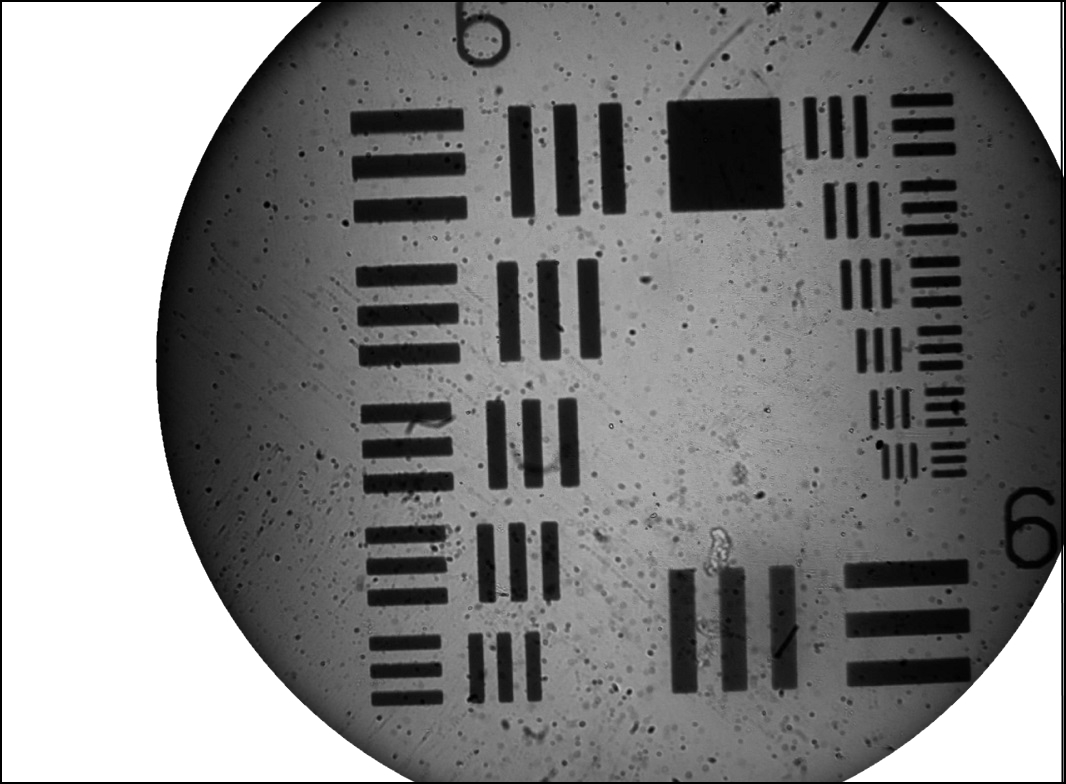
\includegraphics[width=0.7\textwidth,keepaspectratio]{afbeeldingen/process_visibility/m3_bw.jpg}
      \caption{Black and white photo.}
      \label{fig:resolution_target}
    \end{minipage}%
    \begin{minipage}{.5\textwidth}
      \centering
      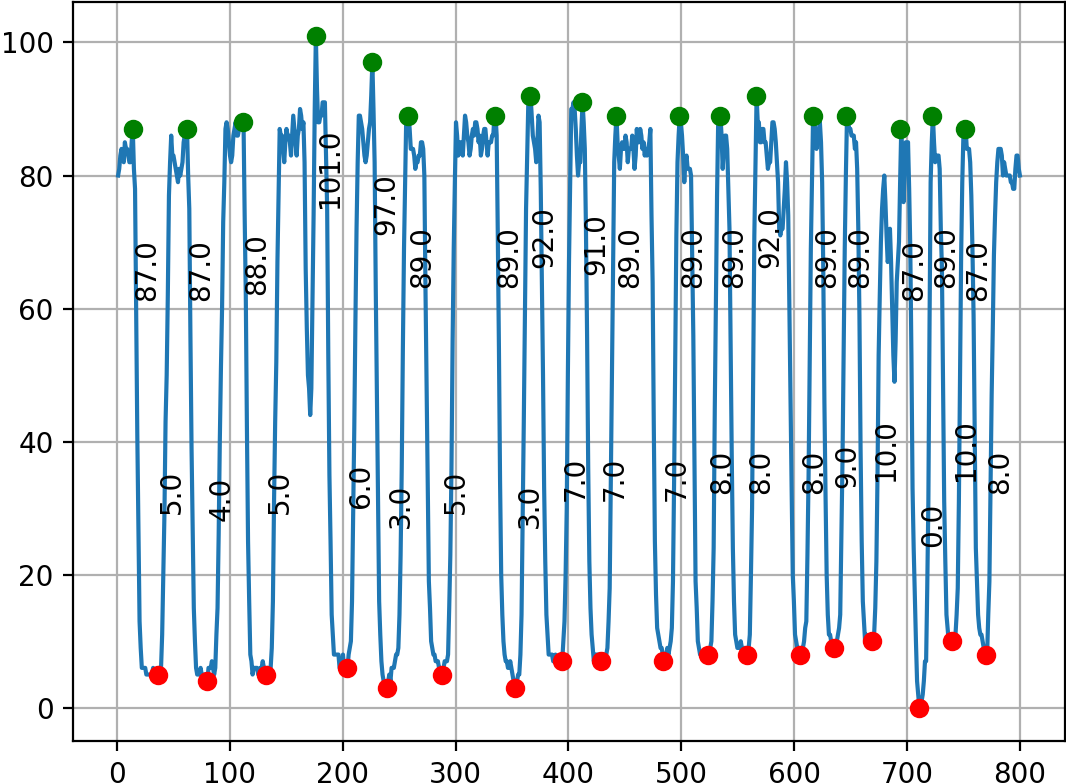
\includegraphics[width=0.7\textwidth,keepaspectratio]{afbeeldingen/process_visibility/m3_rpg_7.png}
      \caption{Linetrace of seventh group.}
      \label{fig:linetrace}
    \end{minipage}
\end{figure}

The high an low values of the line trace were manually read of the photos and entered into a python script capable of calculating the visibility values for each magnification and spatial frequency. The result of which can be seen in figure \ref{fig:visibilities}.\\

\begin{wrapfigure}{l}{0.55\textwidth}
    \centering
    \vspace{-3mm}
    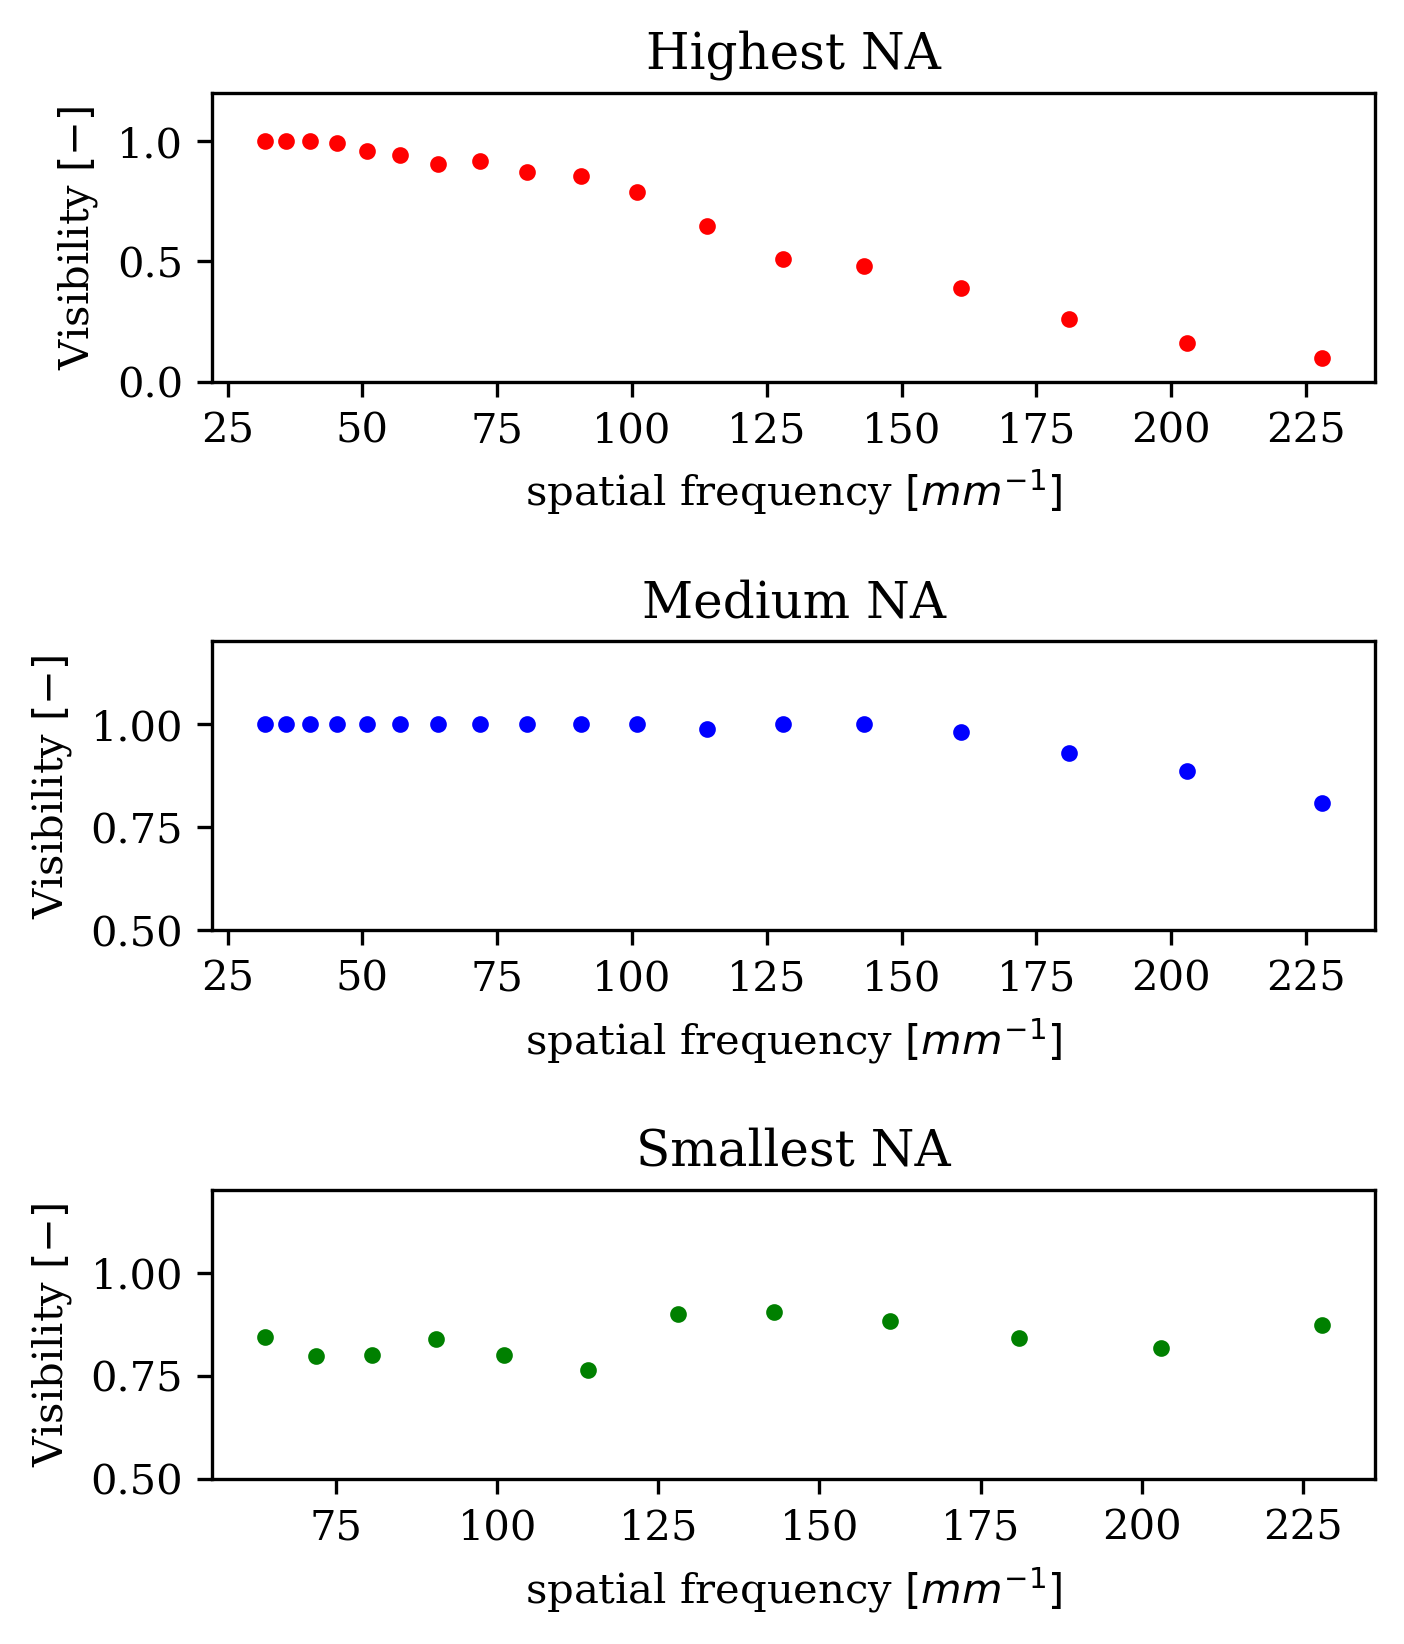
\includegraphics[width=0.55\textwidth,keepaspectratio]{afbeeldingen/visibilities.png}
    \caption{Plots of the visibilities per numerical aperature.}
    \label{fig:visibilities}
    \vspace{0mm}
\end{wrapfigure}

\vspace{-7mm}
The data is plotted in such a way that the highest subplot has the lowest magnification and the lowest subplot has the highest magnification. Each subplot has the dimensionless visibility number plotted on the vertical axis and the spatial frequency plotted on the horizontal axis. We chose this layout since we expect the visibility to decrease when the lines get closer together and the spatial frequency thusly increases. Note that only the verticle visibility axis of the highest subplot starts with a visibility of zero.\\
What we see is not surprising when we also take into account the photos in the appendix. As can be seen on these photos the highest magnification lense has the smallest numerical aperature, therefore all three traced groups are clearly resolvable. Thus the visibility won't drop as much as the lowest magnification lense when the spatial frequency increases.\\
Something noticable however is that the highest magnification plot starts of with the lowest visibility value. This has to do with the fact that this smaller aperature aslo catches less light, the brightest spot in its photo is evidently less bright than that of the other two aperatures. This can be seen when taking a look at either the linetraces or the photos in the appendix.